\lab{Gymnasium}{Gymnasium}

\objective{Gymnasium is a module designed to learn and apply reinforcement learning. 
The purpose of this lab is to learn the variety of functionalities available in Gymnasium and to implement them in various environments.}

Gymnasium is a module used to perform reinforcement learning.
It contains a collection of environments where reinforcement learning can be used to accomplish various tasks.
These environments include performing computer functions such as copy and paste, playing Atari video games, and controlling robots.
To install Gymnasium, simply run the following code:
\begin{lstlisting}
>>> pip install gymnasium 
>>> # You may also need to install these dependencies
>>> pip install gymnasium[all]
>>> pip install gymnasium[classic-control]
\end{lstlisting}

\section*{Environments}

Each environment in Gymnasium can be thought of as a different scenario where reinforcement learning can be applied.
A catalog of environments can be found using the following code.

\begin{lstlisting}
>>> from gymnasium import envs
>>> print(envs.registry.values())
dict_values([EnvSpec(id='CartPole-v0', entry_point='gymnasium.envs.classic_control.cartpole:CartPoleEnv', reward_threshold=195.0, nondeterministic=False, max_episode_steps=200, order_enforce=True, autoreset=False, disable_env_checker=False, apply_api_compatibility=False, kwargs={}, namespace=None, name='CartPole', version=0, additional_wrappers=(), vector_entry_point='gymnasium.envs.classic_control.cartpole:CartPoleVectorEnv'), ...
\end{lstlisting}
To learn more about Gymnasium and its environments, visit \url{gymnasium.farama.org}.

We will demonstrate how to work with Gymnasium environments by walking through the environment \li{"Blackjack-v1"}.
The game Blackjack\footnote{For more on how to play Blackjack, see \url{https://en.wikipedia.org/wiki/Blackjack}.} is a card game where the player receives two cards from a face card deck.
The goal of the player is to get cards whose sum is as close to 21 as possible without exceeding 21.
In this version of Blackjack, an ace is considered 1 or 11 and any face card is considered 10.
On each turn, the player may choose to take another card or stop drawing cards.
If their card sum does not exceed 21, they may take another card, but if it does, they lose.
After the player stops drawing cards, the computer may play the same game.
If the computer gets closer to 21 than the player (without exceeding 21), the player loses.

To begin working in an environment, the environment must be initialized and reset.
Resetting the environment puts everything in the correct starting position and is necessary to begin using the environment.
For example, in \li{"Blackjack-v1"}, restarting the environment deals out a new game of Blackjack.
Once the environment is complete, it should then be closed.
Closing the environment tells the computer to stop running the environment (otherwise it will continue to run in the background).

\begin{lstlisting}
>>> import gymnasium as gym
>>> env = gym.make('Blackjack-v1')  # Initialize Blackjack-v1 environment
>>> env.reset()  # Reset the environment
((16, 6, 1), {})

>>> env.close()  # Close the environment
\end{lstlisting}

\subsection*{Action Space}
Once the environment is initialized and reset, the player can perform actions from the action space.
To perform an action, use the function \li{step()}, which accepts the action as a parameter and returns an observation (more on those later).
Environments may have discrete or continuous action spaces, but the environments presented in this lab all have discrete action spaces.
When the action space is discrete, actions are defined as integers 0 through $n$, where $n$ is the number of actions.
The action each integer represents can be found in the documentation of each environment.
The action space in \li{"Blackjack-v1"} has 2 actions, represented by 0 and 1: 0 indicates that the player will stop drawing cards, and 1 indicates that the player will draw another card.

\begin{lstlisting}
>>> env = gym.make('Blackjack-v1')
>>> env.reset()
((12,9,0),{})
>>> env.action_space  # Determine the number of actions available
Discrete(2)
# Select a random action and take a step using that action
>>> random_action = env.action_space.sample()
>>> random_action 
1
# In this case, the random action was to draw another card
>>> env.step(random_action)
((16,9,0), 0.0, False, False, {})
\end{lstlisting}

\subsection*{Observation Space}
The observation space of an environment contains all possible observations given an action.
For example, in \li{"Blackjack-v1"}, an observation is a tuple containing the total sum of the player's hand, the first card of the computer's hand, and a boolean indicating whether the player has an ace.
The observation from each action can be found in the tuple returned by \li{step()}, which tells us the following information:
\begin{enumerate}
\item \li{observation}: The current state of the environment.
\item \li{reward}: The reward given from the observation. 
In most environments, maximizing the total reward increases performance. 
For example, the reward in \li{'Blackjack-v1'} is 1 if the player wins, -1 if the player loses, and 0 if there is a draw.
\item \li{done}: A boolean indicating whether the observation terminates the environment.
\item \li{truncated}: A boolean indicating whether the episode truncates for an abnormal reason.
\item \li{info}: Various information that may be helpful when debugging.
\end{enumerate}
Consider the code below.

\begin{lstlisting}
>>> env = gym.make('Blackjack-v1')
>>> env.reset()
((12,1,0),{})

>>> random_action = env.action_space.sample()  # Make a random guess
>>> env.step(random_action)
((18,1,0), 0.0, False, False {})
\end{lstlisting}
This tuple can be interpreted as follows:
\begin{enumerate}
\item The sum of the player's hand is 18, the computer's first card is 1, and the player has no ace.
\item The reward is currently 0.0 (the game is not over yet).
\item The environment is not terminated.
\item The episode was not truncated
\item Information that may help debugging (which is currently empty).
\end{enumerate}
In practice, this information is usually accessed by setting variables equal to \li{step()} as in 
\begin{lstlisting}
>>> obs, reward, done, trunc, info = env.step(random_action)
\end{lstlisting}

\begin{problem}
Write a function \li{random_blackjack()} that accepts an integer $n$.
Initialize \\ \li{"Blackjack-v1"} $n$ times and each time take random actions until the game is terminated.
Return the percentage of games the player wins.
Use your function to print the win percentage after 50,000 games.
\label{prob:random-blackjack}
\end{problem}

\section*{Understanding Environments}
Because each action and observation space is made up of numbers, good documentation is imperative to understanding any given environment.
Fortunately, most environments in Gymnasium are very well documented, and most documentation follows the same pattern.
There is a docstring which includes a description of the environment, a detailed action space, a detailed observation space, and explanation of rewards.
It is always helpful to refer to this documentation when working in a Gymnasium environment.

In addition to documentation, certain environments can be understood better through visualization.
For example, the environment \li{"Acrobot-v1"} displays a double pendulum.
Rendering the environment allows the user to see the movement of the double pendulum as forces are applied to it.
The best way to render an environment in Gymnasium is by running the following code through a python (\li{.py}) script, using the argument \li{render_mode='human'}.

\begin{lstlisting}
>>> import gymnasium as gym

>>> env = gym.make('Acrobot-v1', render_mode='human')
>>> # env.reset() returns the observation space and corresponding info
>>> observation, info = env.reset()  

>>> done = False 
>>> while not done:  # Until the environment terminates...
>>>     # Take random step
>>>     random_action = env.action_space.sample()
>>>     obs, reward, done, trunc, info = env.step(random_action)

>>> env.close()
\end{lstlisting}
However, this lab uses a Jupyter (\li{.ipynb}) file, and Gymnasium environments do not render well in Jupyter files.
The visualization technique shown below is a simple workaround that uses the argument \li{render_mode='rgb_array'}, but unfortunately it renders slowly.
\begin{lstlisting}
>>> from IPython import display
>>> from matplotlib import pyplot as plt

>>> env = gym.make('Acrobot-v1', render_mode='rgb_array')
>>> observation, info = env.reset()

>>> # Initialize visualization
>>> img = plt.imshow(env.render())

>>> done = False
>>> while not done:
>>>     # Take random step
>>>     random_action = env.action_space.sample()
>>>     obs, reward, done, trunc, info = env.step(random_action)

>>>     # Update visualization
>>>     img.set_data(env.render())
>>>     display.display(plt.gcf())
>>>     display.clear_output(wait=True)

>>> env.close()
\end{lstlisting}

\begin{figure}[H]

\includegraphics[width=5cm]{figures/acrobot.pdf}
\caption{Rendering of \li{"Acrobot-v1"}}
\end{figure}

\section*{Solving An Environment}

One way to solve an environment is to use information from the current observation to choose our next action.
For example, consider \li{"Blackjack-v1"}.
Each observation tells us the player's current card sum.
Based on the current card sum, we can decide whether we want to draw another card or stop drawing cards.
To take the decided action, simply input the integer representing the action into the function \li{step()}.

\begin{problem}
Write a function \li{blackjack()} which runs a na\"{i}ve algorithm to win blackjack.
The function should receive an integer \li{n} as input.
If the player's hand is less than or equal to \li{n}, the player should draw another card.
If the player's hand is more than \li{n}, they should stop playing.
Within the function, run the algorithm 10,000 times and return the percentage of games the player wins.

For $n=1,2,\ldots,21$, plot the average win rate returned by your function. 
Identify which value(s) of $n$ wins most often.

\noindent Hint: Remember what the actions are in the action space of \li{"Blackjack-v1"}.
\label{prob:blackjack}
\end{problem}

\begin{problem}
The environment \li{"CartPole-v1"} presents a cart with a vertical pole.
The goal of the environment is to keep the pole vertical as long as possible.
The cart moves to the left with action 0, and it moves to the right with action 1.
The observation space of this environment is a 4-dimensional array containing: the cart position, the cart velocity, the pole angle, and the pole angular velocity, respectively.
More information about this environment can be found at \url{gymnasium.farama.org/environments/classic_control/cart_pole/}.

Write a function \li{cartpole()} which initializes the \li{"CartPole-v1"} environment and keeps the pole vertical as long as possible based on the angular velocity of the tip of the pole.
Return the number of steps it takes before it terminates (about 200 on average).

Run the game a single time and render the environment at each step. 
Then run your function 100 times without rendering, and print the average number of steps before it terminates.

\label{prob:cartpole}
\end{problem}

\begin{problem}
The environment \li{"MountainCar-v0"} shows a car in a valley.
The goal of the environment is to get the car to the top of the right mountain.
The car can be driven forward (toward the goal) with action 2, can be driven backward with action 0, and will be put in neutral with action 1.
Note that the car cannot immediately get up the hill because of gravity, so in order to move the car to goal, momentum will need to be gained by going back and forth between both sides of the valley.
The observation space of this environment is a 2-dimensional array containing the $x$ position and the velocity of the car, respectively.
More information about this environment can be found at \url{gymnasium.farama.org/environments/classic_control/mountain_car/}.

Using the given position and velocity of the car, write a function \li{car()} that solves the \li{"MountainCar-v0"} environment.
Return the number of steps it takes before it terminates, which should be less than 180.

Run the game a single time and render the environment at each step. 
Then run your function 100 times without rendering, and print the average number of steps before it terminates.
\label{prob:car}
\end{problem}

\section*{Q-Learning}
While na\"{i}ve methods like the ones above can be useful, reinforcement is a much better approach for using Gymnasium.
Reinforcement learning is a subfield of machine learning where a problem is attempted over and over again. Each time a method is used to solve the problem, the method adapts based on the information gained from the previous attempt.
Information can be gained from the sequence of observations and the total reward earned.

One simple reinforcement method is called \emph{Q-learning}.
While the theory behind Q-learning will not be explained in detail, the main idea is that the next action is not only based on the reward of the current action, but also of the next action.
Q-learning creates a Q-table, which is an $n\times m$ dimensional array, where $n$ is the number of observations and $m$ is the number of actions.
For each state, the optimal action is the action that maximizes the value in the Q-table.
In other words, if I am at observation $i$, the best action is the argmax of row $i$ in the Q-table.

Q-learning requires 3 hyperparameters:
\begin{enumerate}
\item \li{alpha}: the learning rate. This determines whether to accept new values into the q-table.
\item \li{gamma}: the discount factor. The discount factor determines how important the reward of the current action is compared to the following action.
\item \li{epsilon}: the maximum value. This is the max reward that can be earned from a future action (not the current).
\end{enumerate}
These hyperparameters can be changed to create different Q-tables. 
The following function will generate the optimal Q-table for a given environment.

\begin{lstlisting}
def find_qvalues(env, alpha=.1, gamma=.6, epsilon=.1):
    """ Use the Q-learning algorithm to find qvalues.
    Parameters:
        env (str): environment name
        alpha (float): learning rate
        gamma (float): discount factor
        epsilon (float): maximum value
    Returns:
        q_table (ndarray nxm)
    """
    env = gym.make(env)  # Make environment
    # Make Q-table
    q_table = np.zeros((env.observation_space.n, env.action_space.n))

    # Train
    for i in range(1,100001):
        state, info = env.reset()  # Reset state

        epochs, penalties, reward, = 0,0,0
        done = False
        while not done:
            # Accept based on epsilon
            if random.uniform(0,1) < epsilon:
                action = env.action_space.sample()
            else:
                action = np.argmax(q_table[state])

            # Take action
            next_state, reward, done, truncated, info = env.step(action)

            # Calculate new qvalue
            old_value = q_table[state,action]
            next_max = np.max(q_table[next_state])

            new_value = (1-alpha) * old_value + alpha * (reward + gamma * next_max)
            q_table[state, action] = new_value

            # Check if penalty is made
            if reward == -10:
                penalties += 1

            # Get next observation
            state = next_state
            epochs += 1

        # Print episode number
        if i % 100 == 0:
            display.clear_output(wait=True)
            print(f"Episode: {i}")

    env.close()
    print("Training finished.")
    return q_table
\end{lstlisting}

\begin{problem}
The environment \li{"Taxi-v3"} depicts a taxi on a city grid, as shown in Figure \ref{fig:taxi}.
The goal of this environment is to pick up a passenger in a taxi and drop them off at their destination as fast as possible.
You will have to look at the environment specifications at \url{gymnasium.farama.org/environments/toy_text/taxi/} to understand it better.

Initialize the environment, then randomly act until the environment is done and print the total reward.
Since the taxi is acting randomly, it often takes so long for the environment to render that Jupyter will crash, so do NOT attempt to render this environment.

Next, use \li{find_qvalues()} to calculate the optimal Q-table of the environment using \li{alpha=.1}, \li{gamma=.6}, and \li{epsilon=.1}.
Then, render \li{"Taxi-v3"}, use the Q-table to move through it (as described above), and print the total reward.

\noindent Hint: \li{q_table[observation,:]} might be helpful.

Finally, write a function \li{taxi()} which initializes the \li{"Taxi-v3"} environment (without rendering).
Run both scenarios described above $1000$ times each, and return both the average random total reward and the average Q-learning total reward.
\label{prob:taxi}
\end{problem}

\begin{figure}[H]
    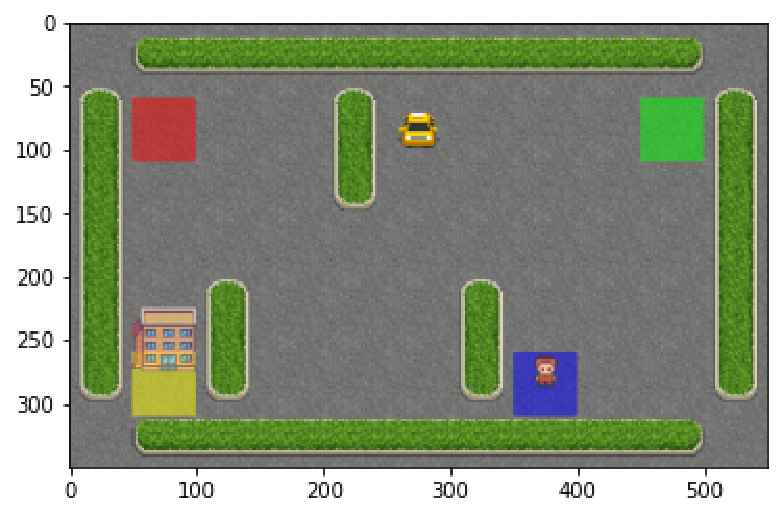
\includegraphics[width=10cm]{figures/taxi.pdf}
    \caption{Example starting position of \li{"Taxi-v3"}}
    \label{fig:taxi}
\end{figure}

